%-----------------------------------------------------------------------------
%  Copyright (C) 2004-2017 Andrew Mathas, University of Sydney
%
%  Distributed under the terms of the GNU General Public License (GPL)
%                  http://www.gnu.org/licenses/
%
% This file is part of the MathQuiz system.
%
% <Andrew.Mathas@sydney.edu.au>
%-----------------------------------------------------------------------------

\synctex=1

\documentclass[svgnames]{article}
\usepackage[a4paper,margin=30mm]{geometry}
\parindent=4mm
\parskip=1mm
\hfuzz 5pt

\usepackage{mathquiz-doc}
\usepackage{xparse}
\usepackage{pdfpages}

\setcounter{secnumdepth}{2}
\setcounter{tocdepth}{2}

\newif\ifCtan\Ctanfalse % condition compilation for ctan distribution

\renewcommand*\contentsname{\relax}

% hyperref links to ctan
\NewDocumentCommand\ctan{ O{pkg/#2} m}{\href{https://www.ctan.org/#1}{\texttt{#2}}}

\newcommand\mathquizopt[1]{\texttt{mathquiz \textemdash\textemdash#1}}

%%%%%%%%%%%%%%%%%%%%%%%%%%%%%%%%%%%%%%%%%%%%%%%%%%%%%%%%%%%%%%%%%%%%%%%%%%%%%%%%%%%%%%%
%% MathQuiz title box for front page
\usepackage{tikz}
\usetikzlibrary{shadows.blur}

\definecolor{stone}{HTML}{E9E0D8}
\tikzset{shadowed/.style={blur shadow={shadow blur steps=5},
                          top color=stone,
                          bottom color=PapayaWhip,
                          draw=SaddleBrown,
                          shade,
                          font=\normalfont\Huge\bfseries\scshape,
                          rounded corners=8pt,
      },
      boxes/.style={draw=Sienna,
                    fill=Cornsilk,
                    font=\sffamily\small,
                    inner sep=5pt,
                    rectangle,
                    rounded corners=8pt,
                    text=Brown,
     }
}

\def\MathQuizTitle{
  \begin{tikzpicture}[remember picture,overlay]
      \node[yshift=-3cm] at (current page.north west)
        {\begin{tikzpicture}[remember picture, overlay]
          \draw[shadowed](30mm,0) rectangle node[Cornsilk]{MathQuiz} (\paperwidth-30mm,16mm);
          \node[Sienna,font=\normalfont\small\itshape] at (\paperwidth/2,2mm)
          {\small \mathquiz{description}};
          \node[anchor=west,boxes] at (4cm,0cm) {\mathquiz{name}};
          \node[anchor=east,boxes] at (\paperwidth-4cm,0) {Version \mathquiz{version}};
         \end{tikzpicture}
        };
   \end{tikzpicture}
}

\hypersetup{pdftitle={MathQuiz manual}}

%%%%%%%%%%%%%%%%%%%%%%%%%%%%%%%%%%%%%%%%%%%%%%%%%%%%%%%%%%%%%%%%%%%%%%%%%%%%%%%%%%%%%%%
%% headers and footers
\makeatletter
\def\@oddfoot{\tiny\MathQuiz -- \mathquiz{version}\hfill\thepage}
\makeatother

\begin{document}

    \MathQuizTitle

    \begin{quote}
      \MathQuiz makes it possible to write on-line quizzes using
      \LaTeX, providing an easy way for anyone who knows \LaTeX\ to
      create an on-line quiz using \LaTeX\ file.  The
      allows the quiz author to concentrate on the content of quizzes,
      unencumbered by the technicalities of HTML and javascript.

     \ScreenShot{quiz-page}

      \begin{center}
        \vskip-10mm
        \begin{minipage}{0.7\textwidth}
          \hspace*{3em}\tableofcontents
        \end{minipage}
      \end{center}

      \bigskip
      \begin{tabular}{@{}ll}
      Authors             & \mathquiz{authors}\\
      Maintainer          & \mathquiz{name}\\
      System requirements & python3 and \LaTeX, including \TeX 4ht and \textsc{make4ht}\\
      Licence             & \mathquiz{licence}\\
      Date                & \mathquiz{release date}
      \end{tabular}
    \end{quote}


    \newpage

\section{Introduction}
    On-line quizzes provide a good way to reinforce learning, especially
    because they can give ``interactive'' feedback to the students based
    on the answers that they give. Unfortunately, in addition to writing
    the quiz content there are significant technical hurdles that need
    to be overcome when writing an on-line quiz -- and there are
    additional complications if the quiz involves mathematics or
    diagrams.

    \MathQuiz makes it possible to write on-line quizzes using \LaTeX,
    which is the typesetting language used by mathematicians and
    educators use \LaTeX\ to write their research papers, books and
    teaching materials.  In principle, the quiz can contain anything
    that can be typeset using \LaTeX.  In practise, the \LaTeX\ is
    converted to HTML using
    \href{https://www.tug.org/applications/tex4ht/mn.html}{\TeX 4ht}
    (and \href{https://github.com/michal-h21/make4ht}{make4ht}), so the
    quizzes can any \LaTeX commands that are understood by \TeX 4ht,
    which is almost everything. In particular, it is possible to use
    graphics constructed using packages like \ctan{pstricks} and
    \ctan{tikz}.

    \MathQuiz supports the following three types of questions:
    \begin{itemize}
      \item Multiple choice questions with a unique correct answer
      \item Multiple choice questions zero or more correct answers
      \item Questions with a numerical answer.
    \end{itemize}
    Each time a student answers a question they are told whether they
    are right or wrong and it is possible for the quiz author to give
    targeted feedback to the student based on their answer.

    The easiest way to explain how \MathQuiz works is by example. The
    following \LaTeX\ file defines a quiz with a single multiple choice
    question that has four possible answers, each of which has a
    customised response.  (Responses to answers are optional, but they
    are one of the main pedagogical advantages of on-line quizzes
    because the quiz can explain to the student why their answer was
    correct or incorrect.)

    \lstinputlisting[style=latexcode]{example}

    Since this is a \LaTeX\ file it can be processed using
    \texttt{pdflatex}, or \texttt{latex}, to produce a readable and
    printable version of the quiz, which can be useful useful when
    proofreading. In this case, the \LaTeX\ version of the quiz looks
    something like this:

    \ScreenShot[0.5]{example1-pdf}

    Of course, the real reason for using \MathQuiz is that it is also
    possible to make an on-line version of the quiz by processing the
    quiz using the \texttt{mathquiz} command. If you do this, and then open
    the resulting web page in your favourite browser, you will see a web page
    that looks something like this:

    \ScreenShot{example-html}

    The on-line version of the quiz displays one question at a time,
    with the question buttons serving the dual purpose of, first,
    providing a way to navigate between the different questions in the
    quiz and, secondly, displaying whether or not the question has been
    attempted and, if so, whether it answered correctly or incorrectly.
    Targeted feedback can be given to the person taking the quiz based
    on their responses.

    As explained in \autoref{S:documentclass}, it is possible to
    customise some aspects of the web pages constructed by \MathQuiz.
    With some rudimentary knowledge of python, it is possible to change the page
    layout of the quizzes or to embed them into your local web pages; see
    \autoref{SS:customisation}.

\subsection{What MathQuiz does and does not do}

    The \MathQuiz program was designed to be run from the command-line,
    so to process the file \textsf{quiz.tex} using \MathQuiz you would
    type

    $>$ \Verb|mathquiz quiz| \qquad or \qquad $>$ \Verb|mathquiz quiz.tex|

    \noindent from the command-line. Although I have not tested this, it
    should also be possible to run \MathQuiz from inside programs like
    \TeX Shop by setting the compiler equal to \textsf{mathquiz}.

    The quizzes made using \MathQuiz are intended to be used as a
    revision resource rather than as an assessment tool. Consequently,
    \MathQuiz does not provide a mechanism for recording the marks
    obtained by the students taking the quiz. Technically, it probably
    would not be very hard to record marks but this introduces a
    significant amount of extra overhead in terms of student
    authentication and interfacing with a database. In addition, if
    \MathQuiz were used as as assessment tool then there would be
    additional ``security issues'' to ensure that the quiz content is
    secure. Currently, even though the solutions to the quiz questions
    do not appear in the HTML source code for the quiz it is possible to
    access the answers if you know when you are doing.

    Each question in a quiz, and each quiz itself, can be attempted as
    many times as the student wants. \MathQuiz does not limit the number
    of times that questions can be attempted.

    The questions in a \MathQuiz quiz are static. In particular, they do
    not accept variables and exactly the same questions will appear in
    exactly the same order each time the quiz is taken. It would not be
    hard to make the questions appear in a random order. Randomising the
    order of the multiple choice answers would be more be difficult with
    the current implementation.

    \MathQuiz is able to ask ``computational'' questions that accept a
    numerical answer, however, symbolic answers are not supported.
    For example, if the answer to a question is $0$ then $\sin(0)$ will
    not be accented as a correct answer and the only way to ask for the
    indefinite integral of a function is as a multiple choice question.

    The quizzes are not timed.

    Some of these issues may be addressed in future releases.

\subsection{Credits}
    \MathQuiz{} was written and developed in the
    \href{http://www.maths.usyd.edu.au/}{School of Mathematics and
    Statistics} at the \href{http://www.usyd.edu.au/}{University of
    Sydney}.  The system is built on \LaTeX{} with the conversion from
    \LaTeX{} to HTML being done by Eitan Gurari's
    \href{http://www.cis.ohio-state.edu/~gurari/TeX4ht/mn.html}{TeX4ht}
    (and, more recently, Michal Hoftich's
    \href{https://github.com/michal-h21/make4ht}{make4ht}.

    To write quizzes using \MathQuiz it is only necessary to know
    \LaTeX, however, the underlying \MathQuiz system actually has three components:
    \begin{itemize}
      \item A \LaTeX{} document class file, \texttt{mathquiz.cls}, and
      a \TeX 4ht configuration file, \texttt{mathquiz.cfg}, that enable the
      quiz files to be processed by \LaTeX{} and \TeX 4ht, respectively.
      \item A python program, \texttt{mathquiz}, that translates the
      \LaTeX{} into xml, using \TeX 4ht, and then into HTML.
      \item Some javascript and css that controls and styles the quiz web page.
    \end{itemize}

   The \LaTeX{} component of \MathQuiz{} was written by Andrew Mathas
   and the python, css and javascript code was written by Andrew Mathas
   (and Don Taylor), based on an initial protype of Don Taylor's from
   2001.  Since 2004 the program has been maintained and developed by
   Andrew Mathas. Although the program has changed substantially since
   2004 some of Don's code and, in particular, his idea of using
   \TeX4ht are still very much in use.

   Thanks are due to Bob Howlett for general help with CSS and, for
   Version~5, to  Michal Hoftich for invaluable technical advice on
   \TeX4ht.

\section{System requirements, installation and configuration}

  \subsubsection{System requirements} Python3 and \LaTeX, including \TeX 4ht
  and \textsc{make4ht}. An up to date distribution of \LaTeX, such as
  that provided by \href{https://www.tug.org/texlive/}{\TeX live}, is recommended.


  \subsubsection{\MathQuiz components}

  The \MathQuiz program has different components:
    \begin{itemize}
         \item \LaTeX\ files (a class file and \TeX4ht configuration files)
         \item Python3 executables that use \TeX4ht to convert \LaTeX\ files into web pages
         \item Web files (javascript and css)
         \item Documentation
    \end{itemize}
  In order for \MathQuiz to work all of these files need to be put in
  appropriate places. Of course, to use the on-line quizzes created by
  \MathQuiz you will also need a web server.  This section guides you
  through what needs to be done.
  \ifCtan
     Fortunately, because \MathQuiz is installed as part of your \TeX\
     distribution, you only need to install the web files used by \MathQuiz
     and this can be done using \MathQuiz.

  \else

  \subsubsection{Installation from zip file}
    The \MathQuiz zip file has three directories, or folders:

    \begin{itemize}
      \item[--] mathquiz/latex
      \item[--] mathquiz/doc
      \item[--] mathquiz/scripts
    \end{itemize}

    The files in the \textsf{latex} directory need to be put somewhere in the \LaTeX\
  search path. For example, on my computer I have these files in

     \Verb|/usr/local/texlive/texmf-local/tex/latex/local/mathquiz|

  After you have moved these files to an appropriate place you will probably need to run
  something like texhash. The exact command that you need to run to tell
  \LaTeX\ that you have installed some files install the latex
  components of the system depends on the \TeX distribution that you are
  using.

  The files in the \textsf{doc} directory are the documentation. You can
  put these files where ever you like!

  The \MathQuiz program itself lives in the script directory. On a unix
  like system I recommend making a link to the file mathquiz.py, which is
  the entry point to the code, using something like:

      \Verb|ln -s <path to scripts directory>/mathquiz.py mathquiz|

  The \textsf{mathquiz} executable should be in the system path.

  It remains to install the web files used by \MathQuiz, which can be
  done using \MathQuiz.
  \fi

  \subsubsection{Installing the web files used by \MathQuiz}
   The quiz files created by \MathQuiz use
   \href{https://en.wikipedia.org/wiki/JavaScript}{javascript} and
   \href{https://www.w3schools.com/css/css_intro.asp}{cascading style
   sheets} (CSS) to render the
   quizzes, so the \MathQuiz javascript and CSS files need to be
   installed on your web server\footnote{In fact, \MathQuiz will work
   even if you do not install these files on your web server, however,
   the quiz pages that it creates will have an annoying message at the
   top of the web page that asks you to install these files.} These
   files can be installed by \MathQuiz using the command:

   $>$ \mathquizopt{initialise}

   \noindent When you run this command you will be prompted for the following:
   \begin{itemize}
     \item The \MathQuiz web directory, which is a directory on your local file system that is visible
           from to your web server
     \item The \MathQuiz URL, which is the \textit{relative} URL to this
     directory that you use to access the files in this directory from
     your browser
   \end{itemize}
   For example, on my system the directory for our web server is
   \textsf{/usr/local/httpd/} and the \MathQuiz web
   files are in the directory \textsf{/usr/local/httpd/MathQuiz}. So, I set:
   \begin{quote}
     \begin{tabular}{lll}
       \MathQuiz web directory &=& \textsf{/usr/local/httpd/MathQuiz}\\
       \MathQuiz relative URL  &=& \textsf{/MathQuiz}
     \end{tabular}
   \end{quote}
   In addition, you can set global defaults for the following.
   \begin{itemize}
     \item department
     \item department\_url
     \item institution
     \item institution
   \end{itemize}
  Leave these blank if you do not want to set defaults for the department and
  institution. You can change these settings at any time using\quad
  \mathquizopt{edit-settings}.

  Once you have run the command \quad\mathquizopt{initialise}\quad to
  copy the \MathQuiz web files onto your web server \MathQuiz is ready
  to use.

\section{The MathQuiz document class}\label{S:documentclass}

This section describes the commands provided by the \MathQuiz document
class for typesetting on-line quizzes. More details and some examples
can be found in the on-line manual in \autoref{S:online}.

\subsection{MathQuiz class options}

\begin{description}
  \item[pst2pdf] If this class option is given then \MathQuiz\ uses
  \ctan{pst2pdf} to convert all postscript objects in the quiz to
  images. This sometimes fixes issues with diagrams drawn using
  \ctan{pstricks}. This class option is equivalent to using
  \mathquiz{pst2pdf} from the command-line.

  \item[tikz] Giving this class option both loads the \ctan[pgf]{tikz} package (so you do
  not need to have \Verb|\usepackage{tikz}| in your \LaTeX\ file) and,
  as a bonus, this option fixes a bug in PGF that
  stops it from working with \TeX 4ht (thanks are due to Michal
  Hoftich!).\footnote{This bug, together with a one-line solution, has
  been reported to the PGF developers but for reasons unknown they have
  not fixed the problem. See
    \href{https://tex.stackexchange.com/questions/386757}{Work around for bug in pgf when used with htlatex}
  for more details.}
\end{description}

All other class options that are given to the \MathQuiz document class
are passed to the \texttt{article} class, which is the base class used
by \texttt{mathquiz}.

\subsection{\MathQuiz commands}
\begin{description}
  \item[$\backslash$BreadCrumb]
     Sets last item in the web page breadcrumb, which refers to the
     current quiz. By default, the breadcrumb is as set to be the
     part of the quiz title, as set by \verb!\title!,
     before the first colon. For example, the title

     \hspace*{20mm}\verb!\title{Quiz 1: Some interesting questions about frogs}!

     sets the breadcrumb to ``Quiz 1''.

  \item[$\backslash$Department]
    The name of the department that runs this unit (for example,
    Mathematics). This appears below the question buttons on the quiz web
    page.

    The department can be set globally using \texttt{mathquiz \textemdash\textemdash edit-settings}.

    Default: \texttt{School of Mathematics and Statistics}

  \item[$\backslash$DepartmentURL]
    The URL for the department that runs this unit. This appears below
    the question buttons on the quiz web page.

    The department URL can be set globally using \mathquizopt{edit-settings}.

    Default: \texttt{http://www.maths.usyd.edu.au}

  \item[$\backslash$Insitution]
    The insitution, or university, that appears below the question
    buttons on the quiz web page.

    The insitution can be set globally using \mathquizopt{edit-settings}.

    Default: \texttt{University of Sydney}

  \item[$\backslash$InstitutionURL]
    The URL for the Institution, or institution, that appears below the
    question buttons on the quiz web page.

    The institution URL can be set globally using \mathquizopt{edit-settings}.

    Default: \texttt{https://www.sydney.edu.au}

  \item[$\backslash$QuizzesURL]
    The URL for the suite of quizzes attached to this unit of study. This
    is used in the breadcrumb at the top of the quiz web page.

    Default: \texttt{Unit code???}

  \item[$\backslash$UnitCode]
    The unit of study code for the course that the quiz is attached
    to. This is used in the breadcrumb at the top of the quiz web page.

    Default: \texttt{Unit code???}

  \item[$\backslash$UnitName]
    The name of the unit of study for the course that the quiz is attached
    to. This is used in the breadcrumb at the top of the quiz web page.

    Default: \texttt{Unit name???}

  \item[$\backslash$UnitURL]
    The URL for the unit of study code for the course that the quiz is attached
    to. This is used in the breadcrumb at the top of the quiz web page.

    Default: \texttt{Unit URL???}

\end{description}

\subsection{\MathQuiz environments }

\subsubsection{Question environments}
\subsubsection{Choice environments}
\subsubsection{Discussion environments}
\subsubsection{Quiz index files}

\section{The MathQuiz program}
\subsection{Command line options}

    The following options can either be used inside \Verb|\MathQuiz| to
    control the formatting \textit{locally} for just the unit being


    \begin{description}
       \item[ -h, --help]            list the command-line options and exit
       \item[-p, --pst2pdf]
          Use pst2pdf to fix issues with images generated by pstricks
       \item[-s,--shell-escape]
          Shell escape for htlatex/make4ht
       \item[--initialise]
          Initialise files and setings for mathquiz
       \item[--settings]
          List system settings for mathquiz
       \item[--edit-settings]
          Edit mathquiz settings
       \item[--build MATHQUIZ\_MK4]
          Build file for make4ht. This can be used to add local
          customisations for make4ht.

       \item[-q, --quiet]
          Suppress tex4ht messages (also -qq etc)
       \item[-l LOCAL\_PAGE, --local LOCAL\_PAGE]
          Local python code for generating the quiz web page
    \end{description}

    \subsection{Local customisation}\label{SS:customisation}

  The "style" of the online quizzes is controlled by the file
  \verb!mathquiz_local.py!. If you want to change the format of the quiz
  pages then the easiest way to do this is to make a copy of
  \verb!mathquiz_local.py!, say to mathquizMyStyle.py, and then edit this file
  directly. To see what the new style looks like you can run the
  mathquiz script with an optional argument that tells mathquiz to use
  your style instead:
  \begin{center}
        mathquiz -l mathquizMyStyle quizfile.tex
  \end{center}
  Using \MathQuiz to regenerate the html files is quite time consuming, so
  while you are editing this file you will find it easier if you ask
  mathquiz not to delete the intermediate files that it creates each
  time. To do this first run mathquiz with the -x option and thereafter
  use -f: mathquiz -l mathquizMyStyle -x quizfile.tex   \# tells
  MathQuiz not to delete intermediate files mathquiz -l mathquizMyStyle
  -f quizfile.tex   \# "fast" option when intermediate files exist Once
  the new page format is finalized it can be made the default by setting
  MathQuizOptions="--local=mathquizMyStyle" at the top of the mathquiz
  shell script.

  The easiest way to change \verb!mathquiz_local.py! is to edit the
  "decorating" html that this file puts around the quiz page. You may
  also need to change the CSS style sheet for mathquiz, which is the file
  web/mathquiz.css. More sophisticated versions of \verb!mathquiz_local.py!
  where you change the underlying python code are of course possible.
  For example, at the University of Sydney our version of this file
  calls our content management system directly and uses this to create
  the web page for the quiz.

\begin{htmlcode}
    quiz_page = r'''<!DOCTYPE HTML>
    <html lang="en-AU">
    <head>
      <title> {title} </title>
      {include}
    </head>

    <body>
      {breadcrumbs}
      {no_script}
      <div class="quiz_page">
        {side_menu}
        {quiz_header}
        <div class="quiz_questions">
          {quiz_questions}
        </div>
      </div>
    </body>
    </html>
    '''
\end{htmlcode}




\section{The on-line manual}\label{S:online}

  \MathQuiz has an \href{http://www.maths.usyd.edu.au/u/MOW/MathQuiz/doc/mathquiz-manual.html}{on-line manual}
  that is written in \LaTeX\ and then
  transformed into a web page using \MathQuiz. The PDF version of this
  manual is included here for your convenience. The source file for the
  on-line manual is included with the documentation of \MathQuiz to
  allow you to create a local versiojn of the on-line manual.

    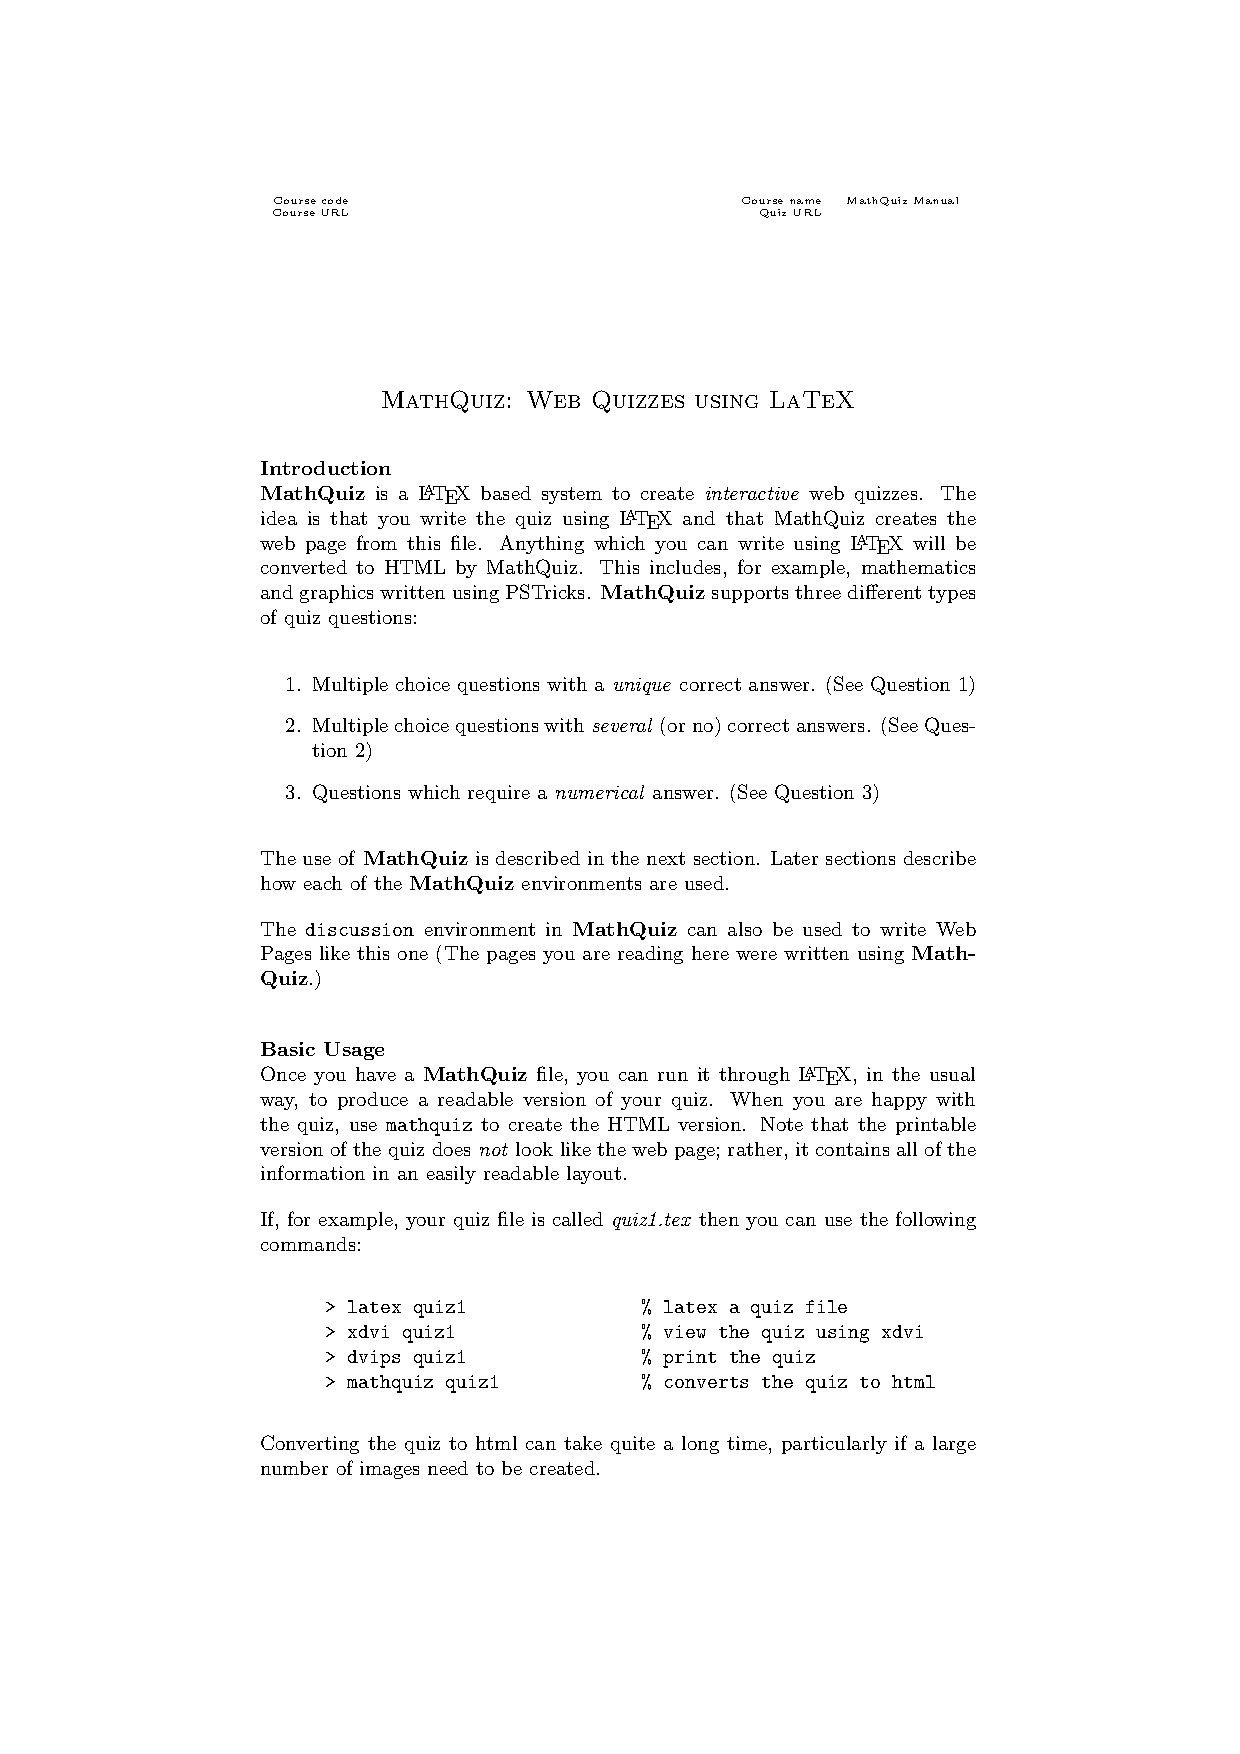
\includepdf[pages=-]{mathquiz-manual}

\section{Licence}

Copyright (C) 2013-2017

\href{https://www.gnu.org/licenses/gpl-3.0.en.html}{GNU General Public License, Version 3, 29 June 2007}

This program is free software: you can redistribute it and/or modify it under
the terms of the GNU General Public License (GPL) as published by the Free
Software Foundation, either version 3 of the License, or (at your option) any
later version.

This program is distributed in the hope that it will be useful, but WITHOUT ANY
WARRANTY; without even the implied warranty of MERCHANTABILITY or FITNESS FOR A
PARTICULAR PURPOSE.  See the GNU General Public License for more details.

\end{document}
